\chapter{Introduction}

\section{Motivation}
\label{sec:intro_overview}
We aim to improve performance and decrease learning times for novice operators of highly complex motor control tasks without increasing cognitive workload.
We are specifically interested in modeling and improving human performance in flight tasks, which generally require extensive training to master.
The Federal Aviation Administration (FAA), for instance, requires a minimum of 1,500 hours as a pilot to captain a U.S. airline~\citep{FAA}.
Being able to decrease this training time could lead to significant cost savings, and the predictive ability provided by modeling human performance could allow for the safer operation of aircraft.

Motor control tasks consist of a wide variety of skills such as playing tuba, pole vaulting, or flying an aircraft.
An individual's performance in any of these skills can change dramatically as they transition from a novice to an expert through training.
We are interested in measuring and modeling this change in performance as it changes over the course of the training process.
We are also interested in developing methods to improve this performance without increasing human workload.

Humans rely on several kinds of feedback during training to improve their performance in motor control tasks.
Feedback can be largely grouped into two types: internal, or intrinsic feedback, and external, or extrinsic feedback.
Intrinsic feedback is anything a person can infer using their own senses: the feel of the valves of a tuba as it is played, the sense of balance mid-jump, or the sound an aircraft engine makes during a climb.
Extrinsic feedback, conversely, is provided by an external source, often in the form of an expert instructor.
Extrinsic feedback comes in many forms and has a long history of improving performance in a large variety of motor control tasks.

We will focus on a specific type of extrinsic feedback known as concurrent bandwidth feedback (CBF), which is a combination of two forms of feedback.
Concurrent feedback is provided in real-time, as an operator is completing a task.
Bandwidth feedback is provided only when a parameter deviates outside a designated range or bandwidth.
Concurrent bandwidth feedback is, therefore, feedback provided to an operator in real-time when a signal deviates out of a predefined range.
This type of feedback has been shown to improve performance in many simple motor control tasks, but has not been investigated in complex, high degree of freedom tasks.
We are interested in measuring, modeling, and predicting the effects of concurrent bandwidth feedback (CBF) on human performance in complex manual control tasks.

It is important to note that this feedback should be thought of as qualitative feedback, not as an additional form of quantitative guidance.
We are not interested in adding additional displays or gauges to control interfaces, but would prefer to modify existing indicators, during training, to better inform an operator as to how well they are performing a task.
Despite extensive evidence demonstrating the effectiveness of this feedback, the mechanism by which it improves performance has yet to be explained or integrated into human performance models.
In this work, we will attempt to explain why concurrent bandwidth feedback is effective in enhancing learning and integrate this explanation into a model.

\section{Background}

\subsection{Augmented Feedback}

% \subsubsection{Augmented Feedback}
The concept of feedback for complex engineering systems was popularized when closed-loop control systems were first developed and has since been redefined many times~\citep{Wierner1948}.
In the context of the current research, a convenient definition of feedback comes from \citeauthor{ramaprasad_definition_1983}, ``[f]eedback is information about the gap between the actual level and the reference level of a system parameter which is used to alter the gap in some way''.
The aforementioned ``gap'' is the error between the current and desired values and can be conveyed to the operator of a system in a variety of ways.
As mentioned previously, feedback can be broadly classified into two types: intrinsic feedback, which is generated from within the context of the action itself, and extrinsic feedback, which is given from an external source~\citep{laurillard_rethinking_2002}.

\begin{figure}[!b]
    \begin{center}
        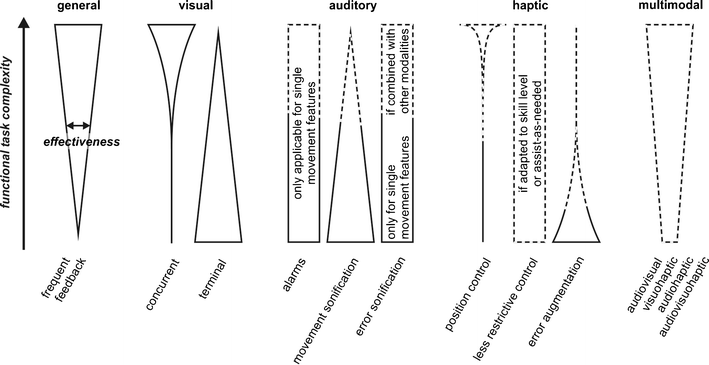
\includegraphics[width=\linewidth]{figures/Introduction/sigrist_review.png}
        \caption[The effectiveness of different types of feedback as a function of functional task complexity]{The effectiveness of different types of feedback as a function of functional task complexity~\citep{sigrist_augmented_2013}. Broader shapes indicate that the feedback is more effective.}
        \label{figure:sigrist_review}
    \end{center}
\end{figure}

Extrinsic feedback, which is also known as augmented feedback, has been extensively studied in the field of motor learning~\citep{sigrist_augmented_2013}.
In their \citeyear{sigrist_augmented_2013} review, \citeauthor{sigrist_augmented_2013} write ``[i]t is generally accepted that augmented feedback, provided by a human expert or a technical display, effectively enhances motor learning.''
There are a variety of forms of augmented feedback that can be further classified by how, when, and what form the feedback is provided.
Each of these choices can significantly impact the effectiveness of augmented feedback, and the summary of \citeauthor{sigrist_augmented_2013}'s review is available in Figure~\ref{figure:sigrist_review}.
Concurrent, or real-time, feedback is displayed to the operator while the task is being executed while terminal feedback, in contrast, is displayed after the task is complete.
Bandwidth feedback is only displayed to the operator when some parameter is inside (on-track feedback) or outside (off-track feedback) of an acceptable, predefined tolerance limit.

Experimentation with bandwidth feedback traces its origins to \citeauthor{thorndike_law_1927}'s \citeyear{thorndike_law_1927} line-drawing experiment.
In his experiment, subjects were seated and blindfolded at a table and asked to draw lines of 3, 4, 5, or 6 inches.
The experiment was divided into two groups of subjects: one group received no verbal feedback, while the other group was told ``right'' if they were within 1/8th of an inch of the desired length for the 3 inch line, or 1/4 of an inch for the other three line lengths, and ``wrong'' if they were outside this bandwidth.
Subjects that received the verbal bandwidth feedback improved from an initial median ``right'' percentage of 13\% to a final ``right'' percentage of 54\% after several training sessions.
The feedback was then removed after these training trials, during which time subjects dropped to a median percentage of 26\%, similar the performance of subjects who never received feedback.
Subjects in \citeauthor{thorndike_law_1927}'s experiments are thought to have become dependent on the verbal feedback (extrinsic feedback) rather than on their visual or proprioceptive sense (intrinsic feedback) to such an extent that they could no longer perform at the previously-demonstrated high levels with the verbal feedback removed.
Similar effects were observed by \citeauthor{kinkade1963differential} in his one-dimensional compensatory tracking task.
In this study, artificial noise was injected into the reference indicator for half of the subjects and half of the subjects were provided audio augmented feedback~\citep{kinkade1963differential}.
He found that augmented feedback always improved performance but that subjects with the artificial noise could not retain this benefit when the feedback was removed.
In the case of \citeauthor{kinkade1963differential}'s work, the artificial noise led subjects to become dependent on the augmented feedback, and they were no longer able to use the intrinsic cues in the task.
This is consistent with the guidance hypothesis (which was not formalized for another fifty years after \citeauthor{thorndike_law_1927}'s experiment was concluded), which states that consistent feedback during the acquisition phase of learning leads to a dependency on that feedback~\citep{salmoni_knowledge_1984}.
Due to this effect, for training to be useful it is important to evaluate augmented feedback in retention to test if subjects are dependent on the extrinsic (augmented) feedback rather than the intrinsic feedback provided by the task.
Care must be taken to design augmented feedback such that it does not block or overshadow the task intrinsic feedback.

\citeauthor{payne_effect_1955} performed one of the first concurrent bandwidth feedback studies in \citeyear{payne_effect_1955}.
In their study, subjects completed a multidimensional pursuit test which required them to scan four simulated aircraft instruments and counter their drift by adjusting simulated aircraft controls.
Subjects were placed into one of three feedback groups: a control level, where no feedback was provided, a second level, which included a single peripheral visual signal when a deviation in one of the displays occurred but did not specify which instrument, and a third level, which provided individual indicators for each of the four instruments and noted the locus of the deviation.
They found a very significant effect between the different feedback groups, with the control group performing the worst, the second level performing better, and the third level performing better still.
Subjects completed the test every hour for a four-hour period.
Performance dropped across all three groups as time elapsed and subjects fatigued, but, despite this fatigue, the performance of the subjects in level three was superior at the end of this period compared to that of the subjects in the control group at the beginning of the experiment.
They concluded by stating that ``the increment is a positive function of the specificity of the information supplied, it can be ascribed largely to the directive properties of the cues, i.e., the cues impose a more efficient temporal and spatial organization upon [the subject's] scanning behavior''~\citep{payne_effect_1955}.

\citeauthor{gordon_effect_1967} performed a rotary pursuit study investigating the effects of on-track and off-track concurrent bandwidth feedback in \citeyear{gordon_effect_1967}.
Subjects in their study were placed into one of three groups: control, on-track feedback, and off-track feedback.
The subjects in the bandwidth feedback groups had to track a 0.75 inch by 0.75 inch target with 0.187 inch rigid stylus tip.
Subjects used the stylus to track the target on a screen, and the position of the stylus and target were recorded.
For subjects in the on-track feedback group, a light bulb was illuminated when they were on target, and for subjects in the off-track group, the light bulb was illuminated when they were not on the target.
While both the on-track and off-track groups performed better than the control group, the off-track group performance was slightly superior.
This finding was consistent with the results \citeauthor{williams_-target_1962} found in a similar task.
Additionally, subjects in the feedback groups completed several trials at the end of the experiment without feedback and did not experience the loss of performance which is often seen due to the guidance hypothesis.
This indicates that subjects were able to use the feedback to better learn the task and were not completely dependent on the feedback.
Subjects used their own intrinsic feedback to learn the task and were able to take advantage of the concurrent bandwidth feedback to better learn and perform the task without becoming dependent on the external feedback.

% Aircraft tasks
\citeauthor{doi:10.1177/107118137802200127} performed two studies to investigate the effects of visual augmented feedback and task difficulty in a two-dimensional pursuit tracking task.
They presented their augmented feedback as additional, continuous displays of task difficulty and performance accuracy in the form of a bar graph.
The performance accuracy augmented feedback was updated in real-time as subjects completed the two-dimensional tracking task, effectively displaying the radial offset between the cursor and target.
In the first of their two experiments, trainees were split into two groups: fixed-difficulty training and adaptive training, where the difficulty of the task gradually increased with trainee skill level.
In each of these groups, half of the subjects received augmented feedback while the other half did not.
In their second experiment, subjects completed adaptive training followed by an adaptive transfer task, and subjects were again split such that they did or did not receive feedback in each part of the experiment.
In their analysis of the results, they concluded that ``visually presented augmented feedback in the form of bar graphs in a two-dimensional pursuit tracking task does not aid tracking performance in training nor transfer'' \citep{doi:10.1177/107118137802200127}.
We hypothesize that subjects either
\begin{enumerate}
    \item did not find feedback useful and ignored it, or
    \item found the feedback useful but over-used it such that they did not attend to the actual task
\end{enumerate}
The first hypothesis is proposed because the additional information provided by the bar charts did not provide the subjects with novel information that they could not directly observe from the primary display.
Translating the error from the visual, two-dimensional information to a one-dimensional bar graph provides less information than one would observe from the primary display.
The perceived workload associated with using this feedback may have been so large that subjects decided to ignore it.
The second hypothesis is that subjects found the feedback so useful that they no longer looked at the actual task, similar to what was observed in our early experiments with augmented feedback~\citep{karasinski_real-time_2016}.
This seems less likely for this case, as the two-dimensional information would not be fully captured by the augmented feedback provided in this study, and subjects would have needed to refer back to the primary display when large errors were presented in the augmented feedback display.
\citeauthor{doi:10.1177/107118137802200127} further surmised that ``the motor skill task used in these studies was too complex to permit the subjects to use the feedback cues provided,'' suggesting that our first hypothesis is more likely.

\citeauthor{doi:10.1177/001872088002200109} has published a number of studies which involved providing supplemental visual cues (augmented feedback) to subjects, who were flight-naive or otherwise in the very early stages of training, to learn to land an airplane~\citep{doi:10.1177/001872088002200109, doi:10.1177/001872089003200305, doi:10.1207/s15327108ijap0702_4}.
Early experiments in \citeyear{doi:10.1177/001872088002200109} showed that an ``adaptive augmented feedback group,'' who were provided additional command guidance cues when deviating from a specified performance envelope, successfully outperformed a control group with only a basic guidance display during retention trials.
The augmented feedback also showed statistically significant improvement in actual aircraft landings conducted with a small number of subjects in a light aircraft.
In \citeyear{doi:10.1177/001872089003200305}, \citeauthor{doi:10.1177/001872089003200305} expanded this work with subjects taking part in a university training program.
In their study, subjects in augmented feedback groups again performed better than a paired student in a control group.
They were able to reduce the effects of individual flight instructors by pairing subjects in the augmented feedback groups and their control group counterpart with the same instructor.
They showed that the adaptive guidance augmentation provided significant performance benefits, and that subjects that trained in their simulator for approximately two hours could reduce their actual flight training time by one and a half hours without any degradation in performance.
Finally, \citet{doi:10.1207/s15327108ijap0702_4} investigated the interaction effect between several variables, including augmented guidance and the quality of scene fidelity.
They showed that augmented guidance again increased flight performance but that this was only the case for low scene fidelity.
This is likely because the ``quality of natural feedback will interact with effectiveness of augmented feedback [such] that augmented guidance would be more useful when the natural feedback was impoverished''~\citep{doi:10.1207/s15327108ijap0702_4}.
In other words, subjects used the augmented feedback less frequently when the visual display of the task was of higher fidelity.
This effect is likely to be highly dependent on the way in which the augmented feedback is presented and represents an interesting opportunity for future work.

A follow-on study to \citeauthor{doi:10.1177/001872088002200109}'s work with augmented feedback and aircraft landing training was completed by \citet{doi:10.1177/0018720809357343}.
They split their subjects into three groups: a control, which received no feedback, a self-controlled, augmented feedback group, and a yoked feedback group.
Subjects in the augmented feedback groups were provided with Precision Approach Path Indicators (PAPIs) in the form of four lights that the subjects were trained to interpret.
Subjects in the self-controlled group could request a PAPI at any time by pressing a button on the controller, after which the PAPI remained on the screen for two seconds.
The yoked feedback group participants were each paired with one member of the self-controlled group and were shown the PAPIs at the same time.
Their results showed that subjects in the self-controlled augmented feedback group performed the best, followed by the yoked and the control groups.
While they theorized that subjects in the self-control group would gradually reduce the number of PAPI requests through training, this was not observed, and subjects tended to request the same number of PAPIs throughout the entire experiment.
Despite this, the performance benefits seen in both the augmented feedback groups persisted in retention trials, suggesting that the guidance hypothesis did not hold in this case.

Recent work in the field has taken advantage of modern computing and sensory-signaling technology to produce higher fidelity simulations.
In \citeyear{de_groot_effect_2011}, \citeauthor{de_groot_effect_2011} investigated the effects of concurrent bandwidth feedback on learning a lane-keeping task in a driving simulator.
Similar to \citeauthor{gordon_effect_1967}, they investigated the effects of on-track and off-track feedback compared to a control group.
Instead of using a visual indicator, however, \citeauthor{de_groot_effect_2011} used haptic feedback in the form of a vibrating chair for their feedback groups.
They found that on-target and off-target groups had better lane-keeping performance than the control group, and that, similar to \citeauthor{gordon_effect_1967} and \citeauthor{williams_-target_1962}, the off-target group performed best.
Retention trials, however, showed that much of this performance improvement was lost when the feedback was removed, which was in accordance with the guidance hypothesis.
Still, some minor performance improvement was retained by the off-target group, which the authors partially attributed to the onset advantage~\citep{fischer_differential_2008}.
The onset advantage ``suggests that the sudden onset of a stimulus is a more powerful perceptual event than a stimulus offset, facilitating low-level perceptual processing and resulting in faster reaction times''~\citep{de_groot_effect_2011}.
This effect could explain a repeated finding that off-track feedback is superior to on-track feedback, even if the effect is generally small.
\citeauthor{de_groot_effect_2011} also measured response time to a secondary task as an estimate of workload but found no differences across groups.

\subsection{SAFER Experiment} \label{safersection}
In order to determine the effects of feedback for training more complex tasks such may be found in human spaceflight, we designed a series of investigations into concurrent bandwidth feedback in a four degree of freedom Simplified Aid for EVA Rescue (SAFER) task~\citep{karasinski_real-time_2016,karasinski_development_2016,karasinski_real-time_2017}.
SAFER is a small, propulsive jet pack worn during U.S. spacewalks for self-rescue in the event of detachment~\citep{Vassigh1998}.
Subjects were tasked with flying a SAFER simulation to perform a virtual inspection of the International Space Station's (ISS) solar arrays.
Subjects were responsible for controlling their three-dimensional position and roll of their jet pack while pitch and yaw were automatically controlled by an autopilot.

Subjects were initially placed 40 feet away from the solar array and were asked to close to 30 feet and hold this distance for the remainder of the task.
They could gauge their distance from the solar array using the indicator on the guidance display and the out-the-helmet display.
Subjects were then asked to inspect four waypoints on the solar array and were given a guidance display for navigation to the waypoints.

\begin{figure}[tb!]
    \begin{center}
        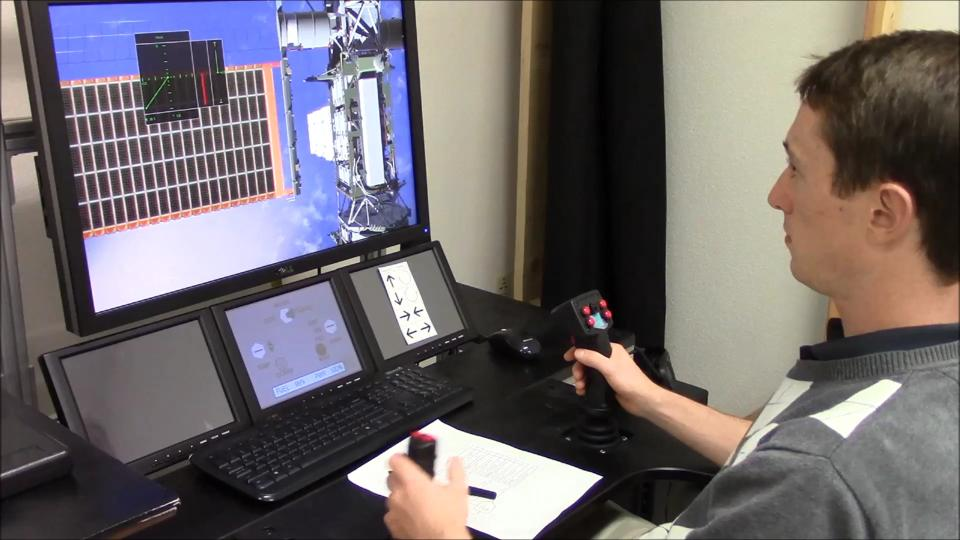
\includegraphics[width=\linewidth]{figures/AR/SAFER_DangerChris.jpg}
        \caption[Simplified Aid for EVA Rescue (SAFER) experiment subject seated in the fixed-base simulator]{A subject from the Simplified Aid for EVA Rescue (SAFER) experiment seated in the fixed-base simulator~\citep{karasinski_real-time_2016}.}
        \label{figure:safersim}
    \end{center}
\end{figure}

Two vertically arranged displays in the simulator were available to complete the task (see Figure~\ref{figure:safersim}).
The primary display contained an out-the-window view of the solar array and, depending on which group the subject was in, one of the guidance displays (see Figure~\ref{figure:safergroups}).
The secondary display, located directly below the primary display, portrayed information about the subject's current mode, remaining fuel, and a ``comm'' light (see Figure~\ref{figure:saferpanel}).
This communication or ``comm'' light on the flight display was used as the secondary task to measure the subject's workload during each trial.
This light was a colored concentric circle on the secondary display and changed from a teal color to a blue or a green color every 5 to 7 seconds (at a pseudorandom interval), and the subjects responded by pressing the corresponding button on the joystick.
This secondary task was displayed on a separate screen from the flight tasks, and the change in color could not be easily distinguished from the subjects' peripheral vision, requiring the subjects to establish a visual scan pattern that included sequential attention to both primary and secondary displays.

\begin{figure}[tb!]
    \begin{center}
        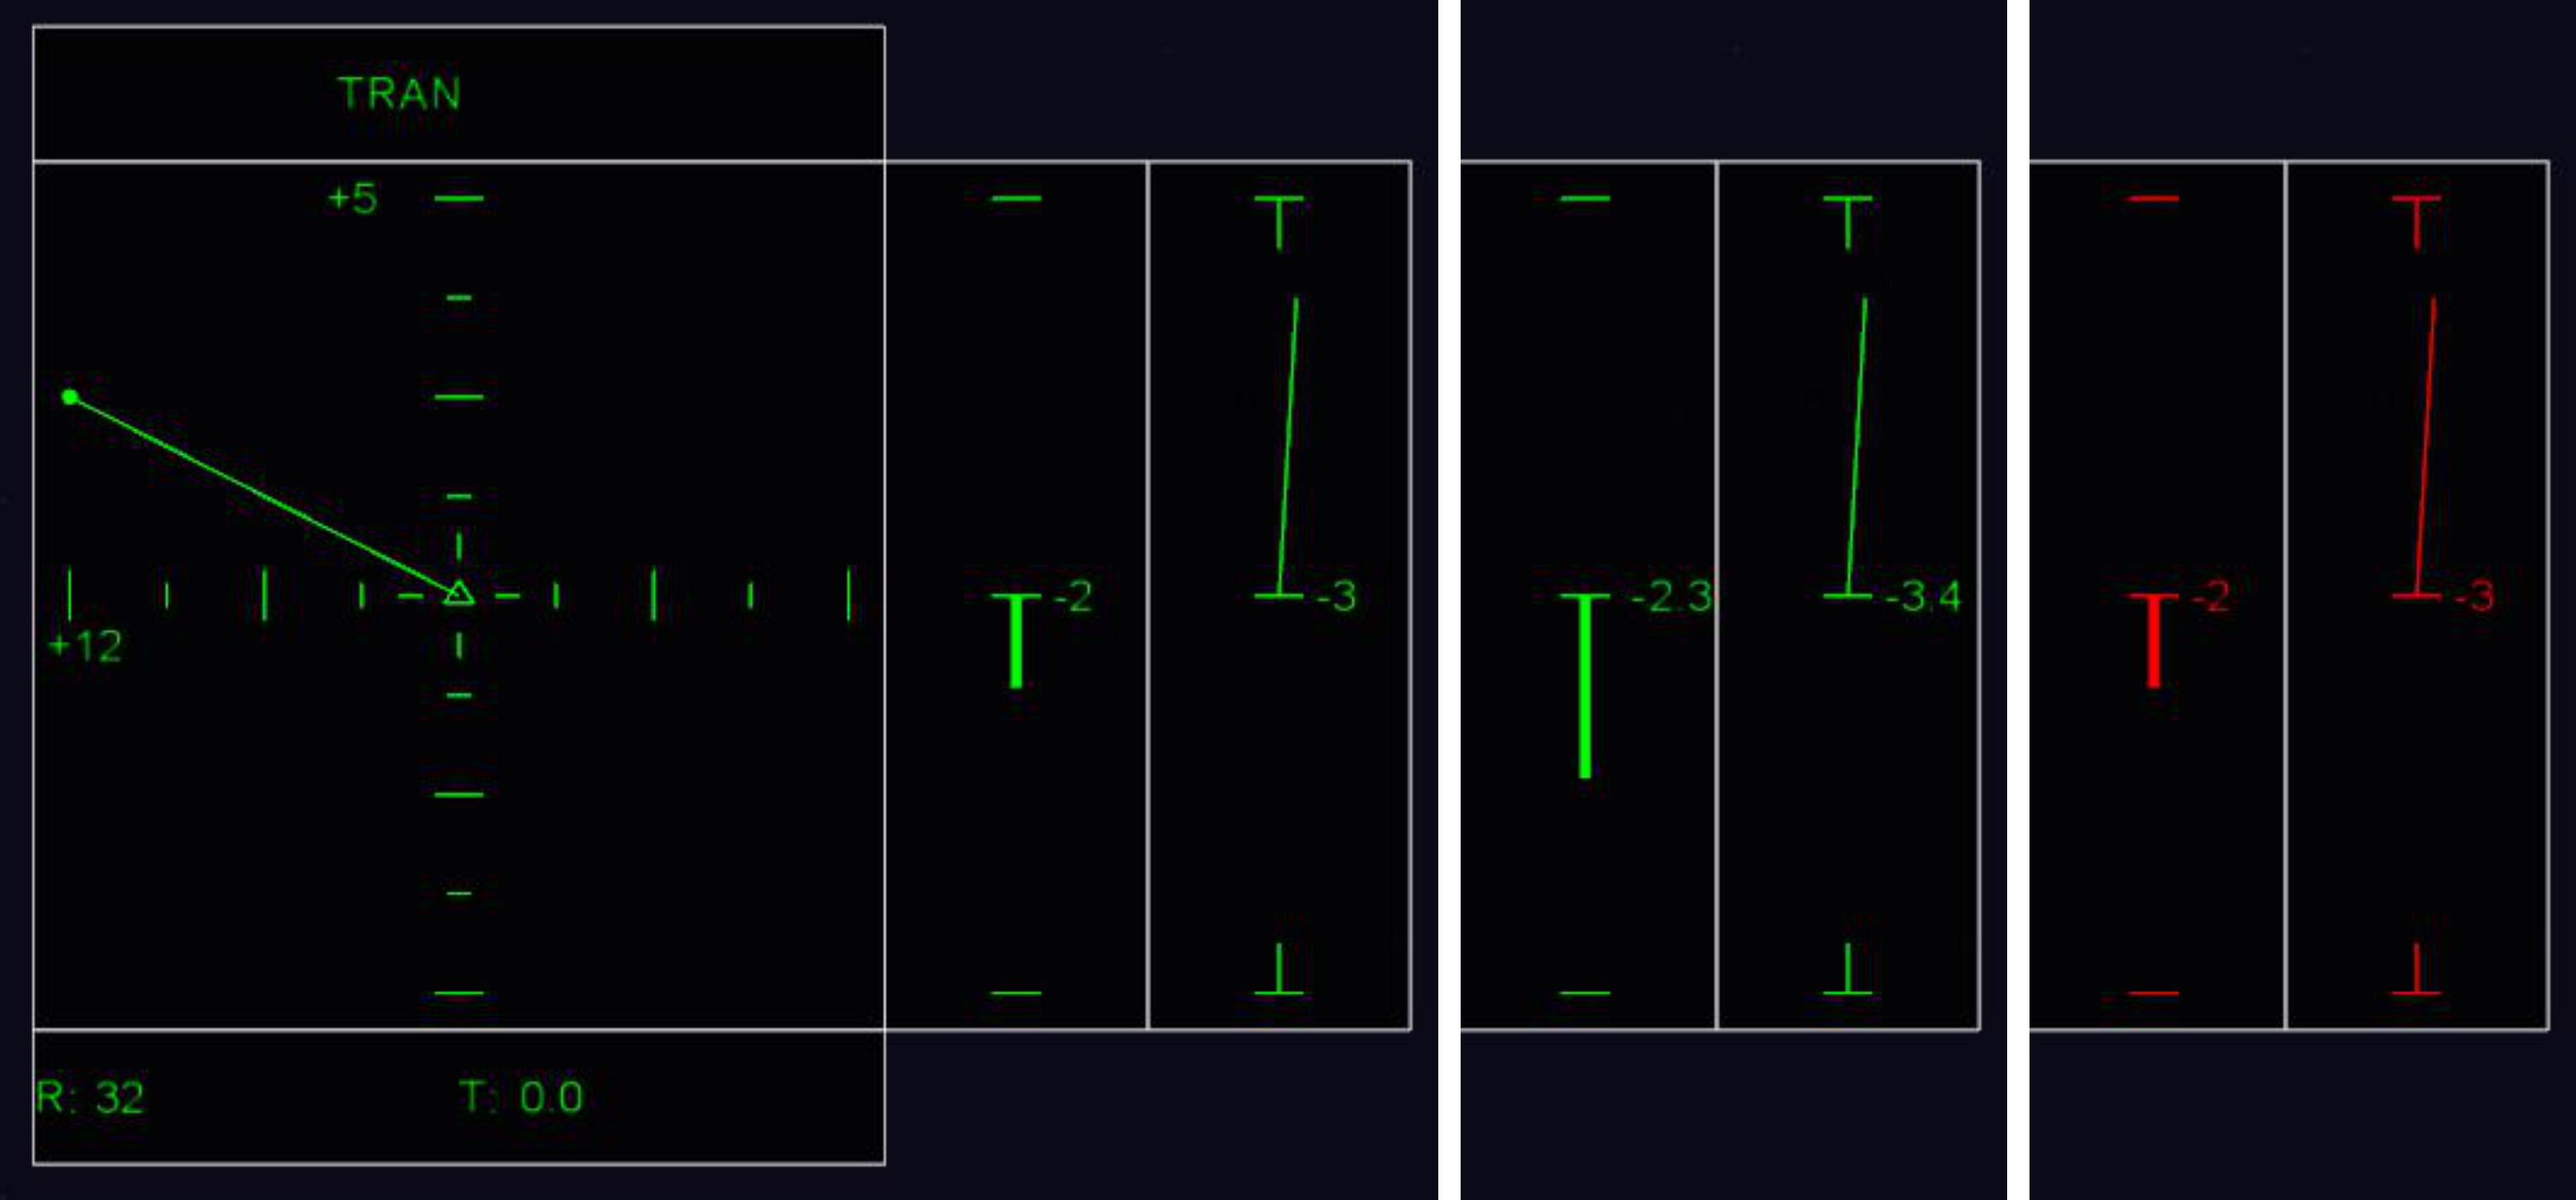
\includegraphics[width=\linewidth]{figures/Introduction/SAFERGroups.png}
        \caption[Simplified Aid for EVA Rescue (SAFER) guidance and feedback display]{Simplified Aid for EVA Rescue (SAFER) guidance and feedback display. The left side of the figure shows the interface presented to the Control, the middle shows the change to the interface for the Precise group, and the right shows the Feedback group's interface when it is activated, while all three groups are in the same state.}
        \label{figure:safergroups}
    \end{center}
\end{figure}

\begin{figure}[tb!]
    \begin{center}
        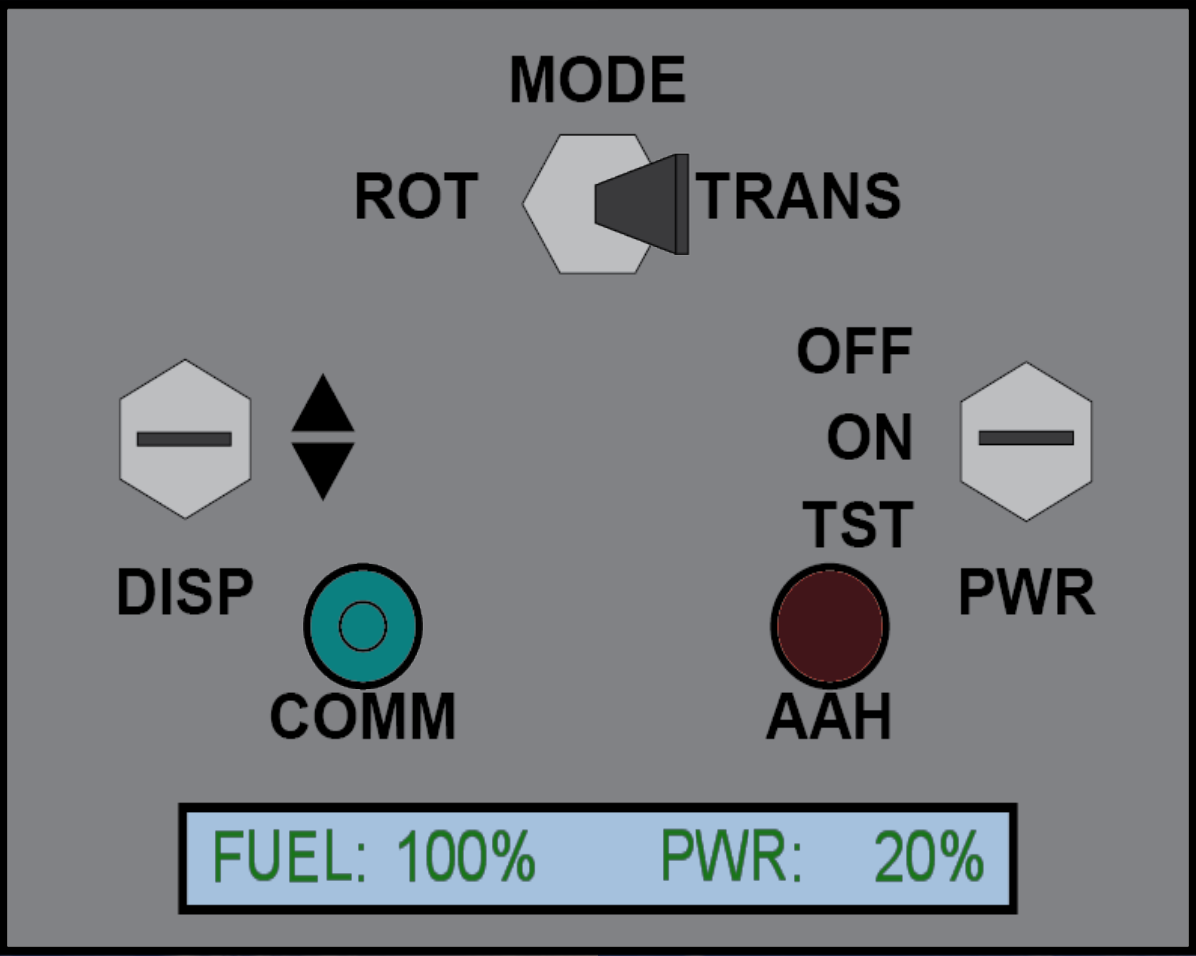
\includegraphics[width=0.8\linewidth]{figures/Introduction/SAFER_Panel.png}
        \caption[Simplified Aid for EVA Rescue (SAFER) secondary display]{Simplified Aid for EVA Rescue (SAFER) secondary display. The current flight mode, remaining fuel and power, and ``comm'' light are all presented.}
        \label{figure:saferpanel}
    \end{center}
\end{figure}

\begin{table}[tb!]
    \centering
    \begin{tabular}{rrrr}
        \toprule
        Name     & Display Max & Sig. Figs & Feedback \\
        \midrule
        Control  & 10 (ft)     & 1         & No       \\
        Precise  & 5 (ft)      & 2         & No       \\
        Feedback & 10 (ft)     & 1         & Yes      \\
        \bottomrule
    \end{tabular}
    \caption[Experimental differences between subject groups]{Experimental differences between subject groups.}
    \label{tab:group_diffs}
\end{table}

In our experiment, subjects were placed into one of three groups: a control, a precise guidance group, and a concurrent bandwidth feedback (CBF) group.
Subjects in the precise guidance group were given an extra significant figure in their guidance display and their analog display was scaled twice as large as the control's (but had half of the maximum value) of their flight parameters.
Subjects in the CBF group had two display elements that would change from a green to a red color when the subject's performance was outside a predefined range.
The two elements represented the distance from the solar array and the roll of the jet pack, and subjects were informed that monitoring and minimizing the error in these variables was their primary task.
The summary of the differences between the three groups are presented in Table~\ref{tab:group_diffs}, and Figure~\ref{figure:safergroups} highlights the interface differences.

Performance was measured as mean absolute distance error (MAE), and results across trials are shown in Figure~\ref{figure:saferdistance}.
Both treatment groups performed better than the control group, with the CBF group performing the best and having the least error.
The treatments had a very different effect on workload than performance, however, and subjects in the precision group reported significantly higher workload than the control group, while subjects in the CBF group reported significantly less workload than the control group (see Figure~\ref{figure:saferworkload}).

The concurrent bandwidth feedback also had the added benefit of significantly reducing the amount of time required to train the subjects to their maximum skill level.
Subjects with the CBF performed better on their first trial than subjects in the control group did on their last, which was after approximately two hours spent training on the task.

\begin{figure}[p]
    \begin{center}
        \begin{subfigure}{0.8\linewidth}
            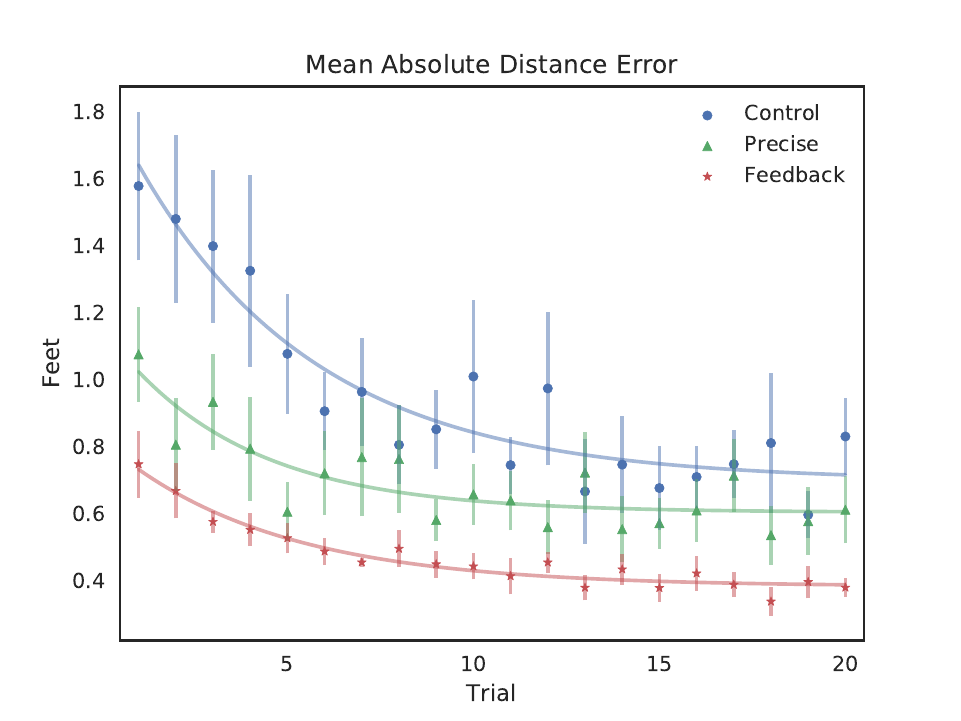
\includegraphics[width=\linewidth]{figures/AR/Group_absDistErr_clean_fit_30.png}
            \caption[Mean absolute distance error]{Mean absolute distance error.}
            \label{figure:saferdistance}
        \end{subfigure}\hfill
        \begin{subfigure}{0.8\linewidth}
            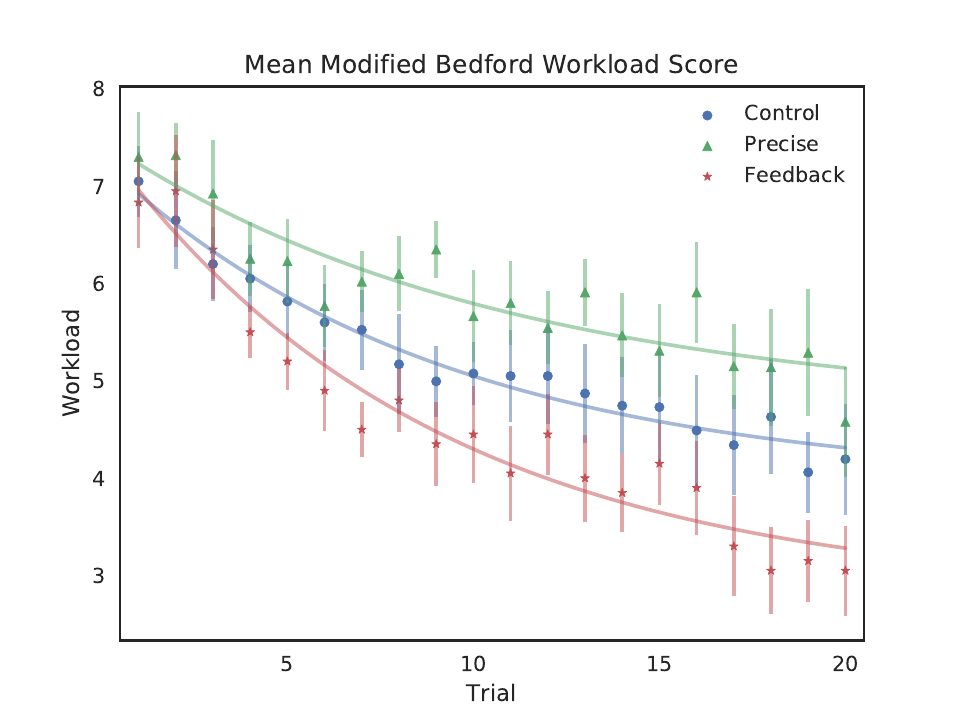
\includegraphics[width=\linewidth]{figures/AR/Group_Workload_fit_30.png}
            \caption[Mean subjective workload rating]{Mean subjective workload rating.}
            \label{figure:saferworkload}
        \end{subfigure}
        \caption[Performance and workload benefits from feedback]{Subjects with concurrent bandwidth feedback (CBF) performed the best (a) and reported the lowest workload (b). Errors are the standard error of the mean~\citep{karasinski_real-time_2016}.}
    \end{center}
\end{figure}

In summary, subjects in the precise and feedback groups had better performance in both the distance and roll tasks than subjects in the control group, and subjects in the feedback group had an initial performance that was superior to the final performance observed by subjects in the control group.
The magnitude of this effect is surprising and appears to confirm that concurrent bandwidth feedback can greatly accelerate the learning of the task.
While subjective workload was not significantly different among the groups, the subjects with feedback also reported the lowest workload.
While presenting more precise guidance information can also improve subject performance, we showed that it does so at the cost of higher workload and longer task completion times compared to the control group.
Concurrent bandwidth feedback was effective at improving subject performance and resulted in subjects reporting lower levels of subjective workload, making it the superior option for training.

\subsection{Concurrent Bandwidth Feedback} \label{section:cbf}

Through our experimental work with augmented feedback, we have found concurrent bandwidth feedback to be an effective technique for enhancing performance without increasing workload.
It is important to carefully consider all aspects of the task when deciding what, when, and how to provide augmented feedback.
While we performed an initial assessment of different whats, whens, and hows when designing the augmented feedback technique presented in this dissertation, we neither completed an exhaustive study, nor did we complete extensive experimental comparisons.
Instead, when designing this feedback, we considered the role of an expert instructor in training a complex skill, such as learning to fly an airplane.
In this instructor model, the trainee has a basic understanding of the task, but the expert instructor can inform them on aspects of the task that they may not be aware of or that they do not have sufficient cognitive margin to attend to.
By pointing at elements on a display or providing minimal verbal feedback, a skilled instructor can call attention to opportunities to improve task execution in real-time with minimal distraction to the student.
The instructor chooses some bandwidth of acceptable performance for each aspect of the task, and their role in providing feedback gradually fades away as the trainee becomes more experienced with the task.
Figure~\ref{figure:afvariables}, adapted from \citeauthor{hodges2020skill}, presents a schematic of the primary what, when, and how variables that need to be considered when providing augmented feedback.
The choices involved in choosing the what, when, and how to provide feedback are presented here.

% WHAT
Deciding \textit{what} information to provide to subjects is not trivial, especially when the task contains a large number of relevant variables.
Under the paradigm of the instructor model, we have chosen to highlight elements that are provided in the guidance display rather than add on additional augmented feedback elements.
\citeauthor{sigrist_augmented_2013} states that ``feedback in complex tasks should be prescriptive--that is, feedback should inform the learning on how to correct the error--rather than descriptive (i.e., information about occurrence of an error)'', even though we have found that purely descriptive feedback can be effective for training complex flight tasks without increasing trainee workload.
Many of the tasks considered by \citeauthor{sigrist_augmented_2013} were targeting specific, short movements or related to sports tasks which do not normally include guidance displays like those found in aerospace tasks.
As these guidance displays are prevalent in the aerospace domain, and our subjects were trained in how to use them to accomplish their tasks, it may be that prescriptive feedback is not necessary in this case.
The subjects are already aware of their errors, and the descriptive feedback provided by the concurrent bandwidth feedback simply provides a description of what the most temporally relevant error is.
It has also been suggested that the motor task is relatively simple for flight and driving tasks and that most of the difficulty associated with the task comes from the high levels of cognitive demand~\citep{doi:10.1080/00222899709600829}.
Under this consideration, simply knowing which error to focus on at any given time may be sufficient for improving performance and could be responsible for the reduction in workload we observed in our previous SAFER study.
In any case, the type of skill and task is certainly ``a critical factor in determining the effectiveness and the appropriateness of the corrective feedback types''~\citep{Tzetzis2008}.

% WHEN
Choosing \textit{when} to provide feedback can be one of the most import aspects of augmented feedback.
Providing feedback terminally, or when the task is over, may be too late to provide a performance benefit, while providing feedback concurrently, in real-time as the task is being executed, can overwhelm the trainee.
\citeauthor{sigrist_augmented_2013} note that ``it seems that the more complex the task, the more the trainee can profit from concurrent feedback.''
When considering the instructor model approach, we chose to focus on concurrent feedback.
% ``Thus, the frequency of feedback should decrease with increasing skill level--that is, with decreasing functional task complexity--to further facilitate motor learning.
% Functional task complexity depends of the current individual skill level and changes during the learning process, whereas nominal task complexity remains invariant.''
It is well established that the frequency of feedback should decrease with increased skill level~\citep{doi:10.1080/00222899809601335, Wulf2002, doi:10.3200/JMBR.36.2.212-224, timmermans_technology-assisted_2009}.
% ``Reduced feedback frequency--that is, fading feedback--seems beneficial for both terminal feedback and concurrent feedback''
It has also been shown that fading feedback, which appears less frequently over time, is beneficial for both terminal and concurrent feedback~\citep{CROWELL201178, KOVACS2011311}.
By reducing the frequency of feedback, subjects learn to develop their internal models of the task and identify their own task errors, reducing their dependency on the feedback.
The role of the instructor should similarly decrease over time as trainees become more proficient.
This conclusion led us to the concept of presenting concurrent feedback when performance variables deviated outside of an acceptable bandwidth.
Bandwidth feedback, however, is not without its own difficulties.
Several authors have noted that ``[b]andwidth feedback has been shown to be effective; however, setting the error threshold is not trivial''~\citep{timmermans_technology-assisted_2009, RIBEIRO2011231, sigrist_augmented_2013}.
This issue has usually been associated with terminal bandwidth feedback, where it is challenging to decide what types of descriptive summary statistics are appropriate and what bandwidths are sufficient.
By instead choosing to present the feedback concurrently we can use an operational limit or chosen bandwidth of acceptable performance, which can make the choice of setting the error threshold simpler.

% HOW (and where)
The \textit{how} of presenting feedback has largely focused on which modality (or modalities) to use.
Under the paradigm of the instructor model, we considered the verbal and visual modalities.
Many aerospace tasks, however, involve significant secondary tasks in the form of managing interactions with air traffic control or communicating over other voice loops.
To avoid interference and competition with these tasks, the concurrent bandwidth we developed was exclusively visual, involving color changes on the guidance display.
One advantage of focusing on the visual modality is that this is where a majority of research in augmented feedback has focused, allowing us to compare between other research studies more easily.

\begin{figure}[tb]
    \begin{center}
        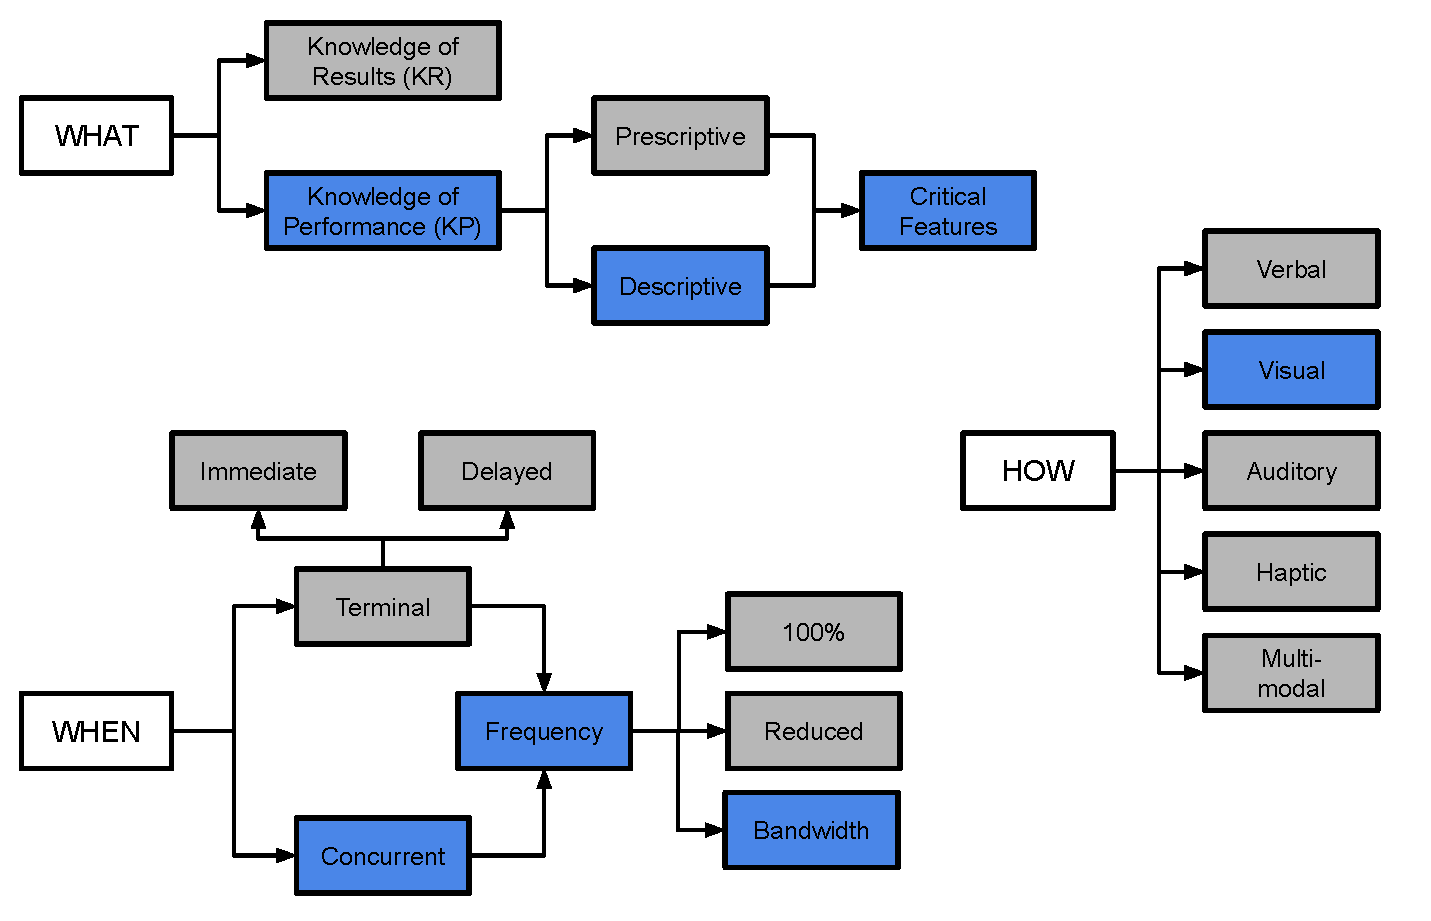
\includegraphics[width=\linewidth]{figures/Introduction/feedbackschematichighlighted.pdf}
        \caption[A schematic of the primary what, when, and how variables that need to be considered when providing augmented feedback]{A schematic of the primary what, when, and how variables that need to be considered when providing augmented feedback, adapted from~\citep{hodges2020skill}. Blue boxes identify the primary feedback considered in this dissertation.}
        \label{figure:afvariables}
    \end{center}
\end{figure}

In summary, concurrent bandwidth feedback is provided to an operator in real-time when a signal deviates out of a predefined range.
In this work, the feedback is always displayed visually and changes the color of an already existing element of the display.
Figure~\ref{fig:cbf} illustrates the process of taking the signal from a task relevant feature and applying this technique.
For example:
\begin{enumerate}
    \item A task relevant signal is identified.
          Figure~\ref{fig:signal} shows an example signal, the pitch disturbance from the aircraft flight task presented in Chapter~\ref{chapter:aircraftfeedback}.
    \item An operationally relevant performance bandwidth is identified.
          Figure~\ref{fig:signal_w_bandwidth} shows an example bandwidth of acceptable performance.
    \item Visual feedback is applied to an existing part of the display and is presented to the operator concurrently.
          Figure~\ref{fig:signal_w_feedback} shows an example of feedback that would be presented to an operator.
          In this example, an element of the display would change from green (acceptable performance) to red (unacceptable performance) when the operator deviates outside of the acceptable pitch range.
\end{enumerate}

\begin{figure}[p]
    \begin{center}
        \begin{subfigure}{0.7\linewidth}
            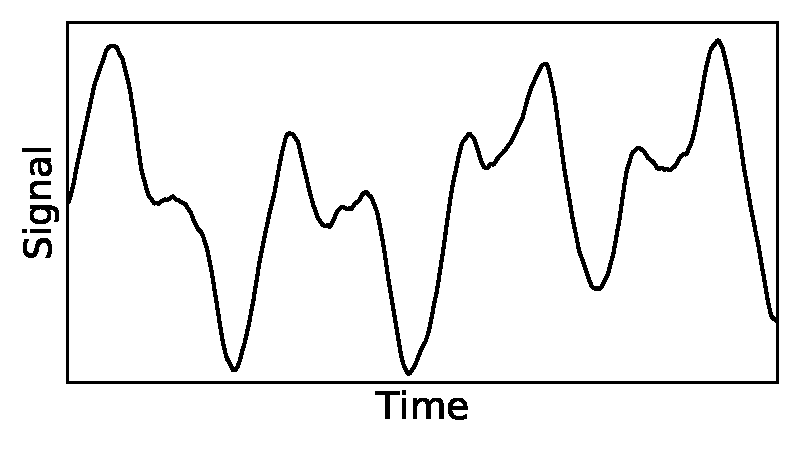
\includegraphics[width=\linewidth]{figures/Introduction/signal.pdf}
            \caption[The signal of a task critical feature]{The signal of a task critical feature.}
            \label{fig:signal}
        \end{subfigure}\hfill
        \begin{subfigure}{0.7\linewidth}
            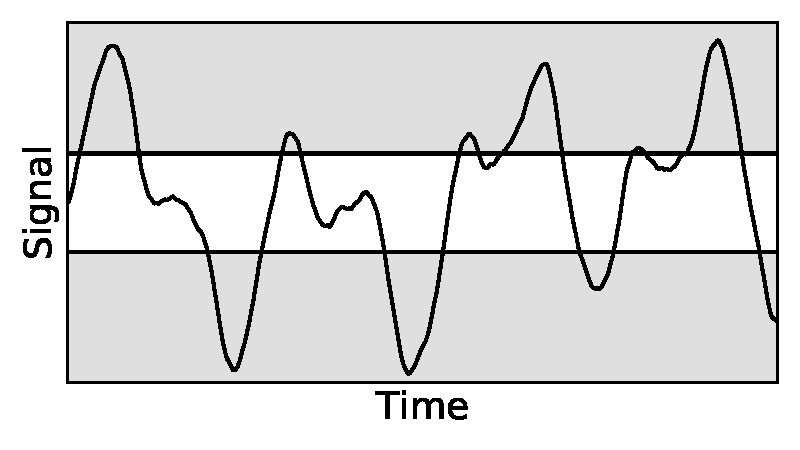
\includegraphics[width=\linewidth]{figures/Introduction/signal_w_bandwidth.pdf}
            \caption[The signal with an operationally relevant bandwidth]{The signal with an operationally relevant bandwidth.}
            \label{fig:signal_w_bandwidth}
        \end{subfigure}\hfill
        \begin{subfigure}{0.7\linewidth}
            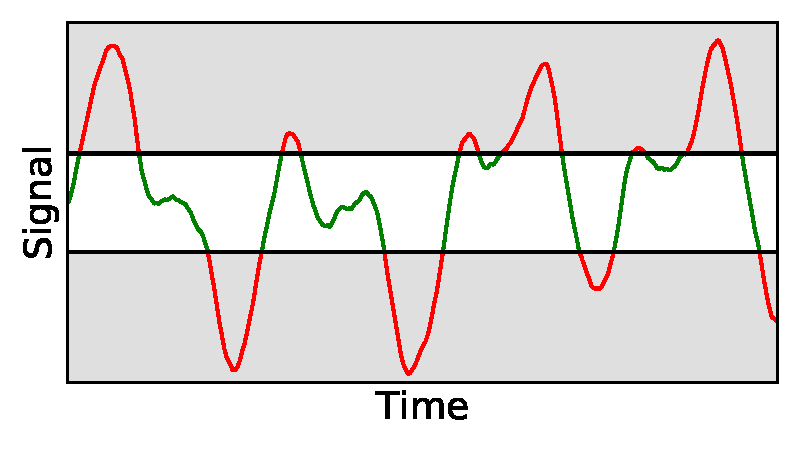
\includegraphics[width=\linewidth]{figures/Introduction/signal_w_feedback.pdf}
            \caption[The signal with concurrent bandwidth feedback applied]{The signal with concurrent bandwidth feedback applied.}
            \label{fig:signal_w_feedback}
        \end{subfigure}
        \caption[The implementation of concurrent bandwidth feedback to the signal of a task critical feature]{The implementation of concurrent bandwidth feedback to the signal of a task critical feature.}
        \label{fig:cbf}%
    \end{center}
\end{figure}

\subsection{Workload}
Improved performance, through some kind of feedback or other technique, often comes at the cost of increased workload, which can lead to a loss of the ability to maintain high performance over a sustained time frame due to fatigue~\citep{karasinski_real-time_2016}.
While improving performance is the most common motivator for supplying augmented feedback, the workload of subjects must also be considered.
If performance benefits come at the cost of increased or unsustainable workload levels, for instance, the cost of augmented feedback may be too high.
For this reason, we are interested in measuring the workload associated with participants to evaluate if including concurrent bandwidth feedback has a net positive effect.

In the human factors community, one of the challenges associated with measuring workload has been the inability to agree on a single definition of the term.
As \citeauthor{hart_nasa-task_2006} notes in her \citeyear{hart_nasa-task_2006} report, ``[t]he many definitions [of workload] that exist in the psychological literature are a testament to the complexity of the construct''.
Workload has been defined by \citeauthor{hart_development_1988} as ``the perceived relationship between the amount of mental processing capability or resources and the amount required by the task.''
\citeauthor{hart_nasa-task_2006} later provided an excellent definition of workload that is broadly acceptable for many types of tasks, ``[w]orkload is a term that represents the cost of accomplishing mission requirements for the human operator''.
More specific definitions are available when focusing in the aerospace domain.
After sending a questionnaire to some 350 military and airline pilots, \citeauthor{ellis1982airline} analyzed the results and proposed that ``[p]ilot workload is the integrated mental and physical effort required to satisfy the perceived demands of a specified flight task''.
% This definition notes three distinct sources of workload: mental effort, physical effort, and task demands.
Regardless of the precise definition, is generally agreed that having a low workload indicates that it would be easy to complete additional tasks, while having a high workload suggests that it would be difficult.

While there are several objective techniques that attempt to capture workload, the most commonly used techniques are subjective in nature~\citep{hart_development_1988}.
In the domain of aircraft flight tasks, the two most commonly used subjective workload measurements are the Modified Bedford Workload Scale and the NASA Task Load Index (NASA-TLX)~\citep{roscoe_subjective_1990, hart_development_1988, hart_nasa-task_2006}.
Both techniques are used in the studies presented in this dissertation and generally show good agreement for the types of tasks that we are interested in.

The Modified Bedford Workload Scale is a 10-point scale that asks operators to rate their spare time to attend to additional tasks.
While taking the survey, operators ask themselves a series of questions to determine if the workload for the task was satisfactory, tolerable, possible, or impossible.
The scale ranges from a score of 1 (a ``piece of cake'') to a 10 (adequate performance was impossible), see Figure~\ref{figure:modifiedbedford}.
The benefits of this scale include that the resulting workload score is a single number which can be easily analyzed statistically, that it is extremely quick to complete, and that it is easy and intuitive for inexperienced subjects to complete.
Some of the negative features of the scale are that it only considers the amount of spare cognitive ability to attend to additional tasks and that there can be large inter-rater variability.
Despite this, the scale is widely used for measuring the workload associated with aircraft flight tasks and has significant heritage in the aerospace domain.

The NASA Task Load Index (NASA-TLX) is one of the best-known and commonly used subjective workload measures.
The NASA-TLX has been in use for thirty years and has been validated over a large variety of tasks~\citep{hart_nasa-task_2006}.
The NASA-TLX is a multidimensional rating scale which uses the magnitude and ranking of six subscales to produce an overall estimate of subjective workload~\citep{hart_development_1988}.
The six subscales are: Mental Demand, Physical Demand, Temporal Demand, Performance, Effort, and Frustration, see Figure~\ref{figure:nasa-tlx}.
Each of these scales is rated on a 0 (Very Low) to 100 (Very High) scale, with the exception of Performance, which is rated from 0 (Perfect) to 100 (Failure).
After marking a value for each of these subscales, subjects then make fifteen pairwise weightings, allowing them to rate each pair of subscales based on its perceived contribution to their overall workload.
A final, overall workload score is computed by multiplying each subscale's score by the number of times it was chosen in the pairwise weightings, adding these values, and dividing by fifteen.
As certain subscales may be more or less important than others, depending on the task being evaluated, researchers can omit subscales or simply not compute the overall score.

In addition to subjective measures of workload, there are a variety of techniques which aim to estimate objective workload.
One of the most common objective measurement techniques is the secondary task, which requires subjects to complete the primary task then use any spare cognitive margin to respond to an additional task~\citep{gawron_human_2008}.
Secondary tasks can provide a measure more sensitive to differences in workload and performance than a single task alone and allow for a common measure between experimental conditions~\citep{slocum1971meaningful}.
Care must be taken, however, to ensure that the secondary task does not intrude upon primary task performance~\citep{williges_behavioral_1979}.
It is important that the secondary task requires a relatively small percentage of the overall cognitive margin compared to the main task, otherwise the distinction between primary and secondary task begins to blur.
In our previous studies, we have used a multiple-choice reaction time task as an objective workload measurement.
In this multiple-choice secondary task, subjects are presented with several different stimuli, each of which requires a different response~\citep{lysaght_operator_1989}.
A subject's objective workload can then be inferred by either the percentage of secondary tasks which were correctly responded to within a given time, the number of secondary tasks which were correctly responded to in a trial, or both.
We have previously found this type of task to be correlated with subjective workload scales in the aforementioned SAFER task~\citep{karasinski_real-time_2017}.
This secondary task approach does not work well for simple tasks, as completing it begins to compete for attention with the primary task but works well for more complex tasks and so is a valid technique for our interests.

\subsection{Pilot Modeling}
\label{background:pilotmodeling}

\begin{figure}[!b]
    \begin{center}
        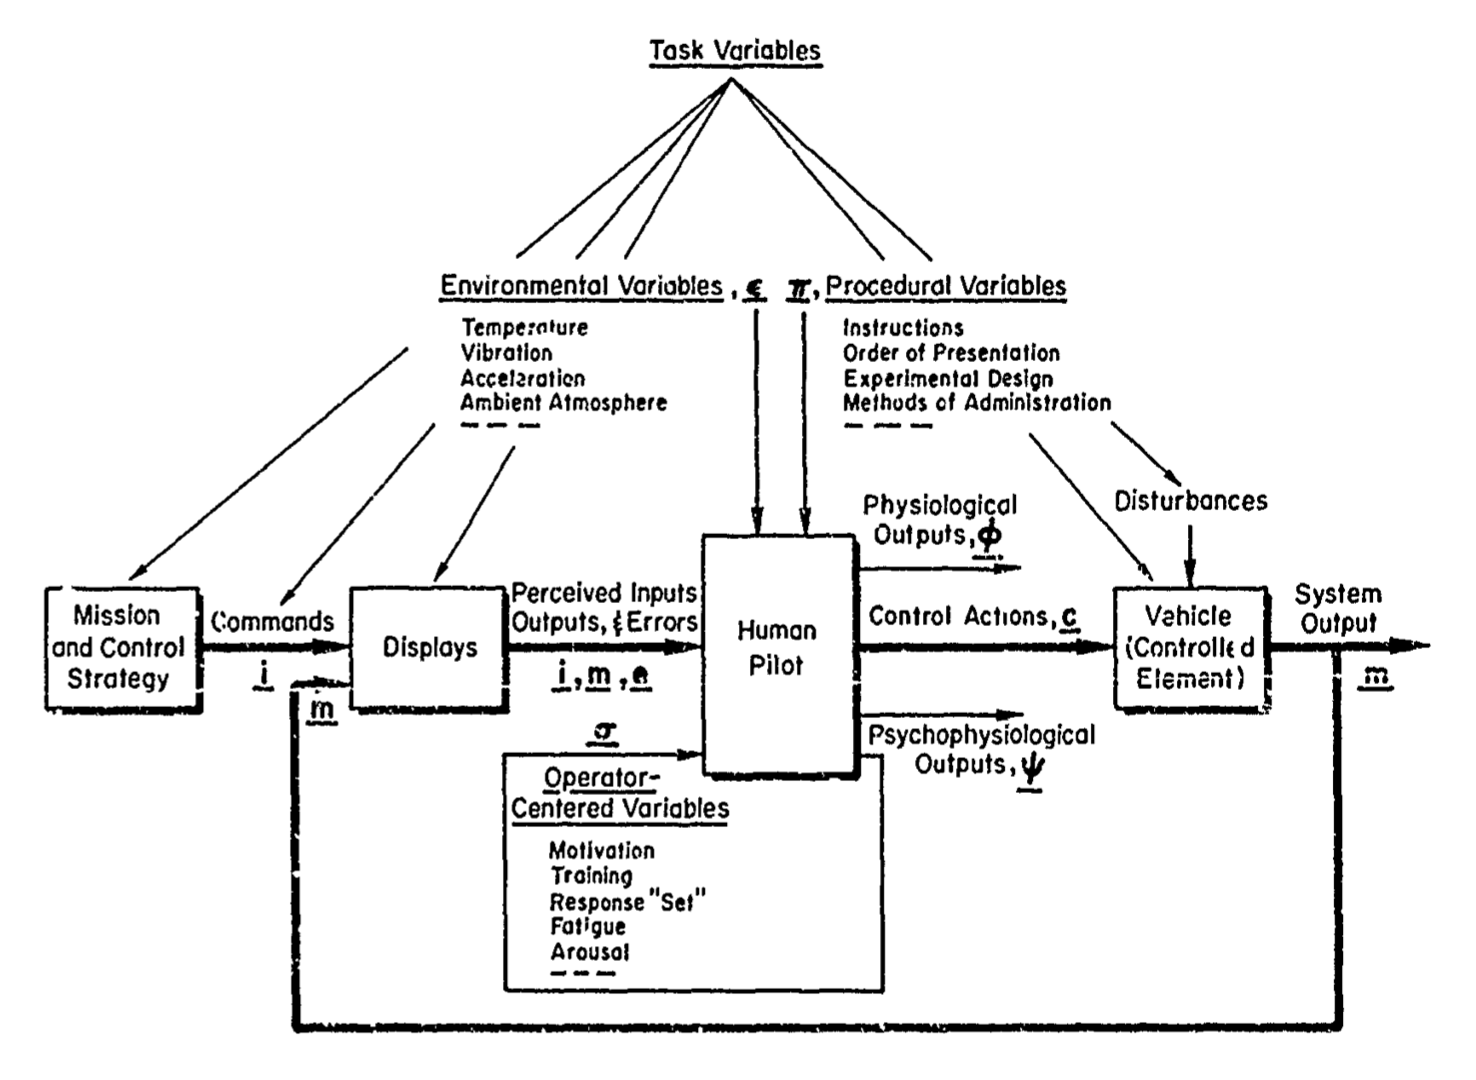
\includegraphics[width=0.8\linewidth]{figures/Introduction/Screen_Shot_2018-07-25_at_10_37_08_AM.png}
        \caption[Variables affecting the pilot/vehicle system]{Variables affecting the pilot/vehicle system, from~\citet{mcruer_mathematical_1974}.}
        \label{figure:mcruer1974}
    \end{center}
\end{figure}

In addition to popularizing the concept of feedback, the creation of control theory in the early 1940s also provided the tools required for the mathematical modeling of the human pilot.
At that time, new weapons were being created for World War II that could only be used effectively with trained operators working with a machine.
While it was thought that a human could be viewed as a unique kind of servomechanism in the control feedback loop, it was still unclear what factors affected human performance.
Early work by Tustin and others extended the control theory framework and applied these theories to actual human operators~\citep{tustin1944investigation}.
Significant attention was focused on ``attempt[ing] to find the laws of relationship of movement and error.
In particular, it was hoped that this relationship [would] be approximately linear and so permit well developed theory of `linear servomechanisms' to be applied to manual control in the same way as it applies to automatic following''~\citep{tustin1944investigation}.
This would allow for the prediction of human performance and the ability to predict the limits of human control.

These early works were summarized in \citeauthor{mcruer_dynamic_1957}'s report, ``Dynamic Response of Human Operators.''
This work evaluated measurements for single-input/single-output (SISO) manual control systems and developed predictive models consistent with this data.
Indeed, \citeauthor*{mcruer_dynamic_1957} wrote, ``[i]t is possible, without doing violence to the data, to obtain describing functions which are generally applicable to the results of the many diverse experiments.''
The report concludes by describing a hypothetical transfer function of the human operator which includes a time delay, a neuromuscular lag, and a gain.
McRuer's early model of the complete pilot/vehicle system is presented in Figure~\ref{figure:mcruer1974}.
McRuer revisited these results in \citeyear{mcruer_mathematical_1974} after two decades of supporting engineering and experimental psychology experiments and was able to further generalize these results to a wide variety of system dynamics.
In his study, McRuer completed a detailed analysis which included the human response to proportional, rate/velocity, and acceleration type controlled element dynamics (see Table~\ref{table:mcruer1974a}).
The result of this report was the now famous ``crossover model,'' which relates the operator and controlled element transfer characteristics by the equation
\begin{align}
    Y_c(jw) Y_p(jw) = \dfrac{w_c e^{-jw \tau_e}}{jw}
\end{align}
where $Y_c$ is the controlled element transfer function, $Y_p$ is the approximate human operator transfer function, $w_c$ is the crossover frequency, and $\tau_e$ is the effective time delay of the pilot.
The crossover model is so named as it allows for linear behavior at approximately -20 dB/decade slope in the region of the crossover frequency.
The approximate human operator response to several controlled element transfer functions and their combined open-loop transfer function are presented in Table~\ref{table:mcruer1974b}.
Modeling the human pilot with the crossover enabled a more complete view of the pilot/vehicle system and allowed for human factors recommendations towards the design of new vehicles.
Even today, the crossover model is used as the standard for describing pilot/vehicle systems at the crossover frequency~\citep{mcruer_human_1965, mcruer_mathematical_1974, xu_review_2017}.

\begin{table}[tb]
    \centering
    \includetable{intro-idealized-control-elements.tex}
    \caption[Example Applications of Idealized Controlled Element Forms]{Example Applications of Idealized Controlled Element Forms, adapted from~\citet{mcruer_mathematical_1974}.}
    \label{table:mcruer1974a}
\end{table}

\begin{table}[tb]
    \centering
    \includetable{intro-human-operator-characteristics.tex}
    \caption[Summary of Human Operator Approximate Characteristics]{Summary of Human Operator Approximate Characteristics, adapted from~\citet{mcruer_mathematical_1974}.}
    \label{table:mcruer1974b}
\end{table}

The continued demand for human pilot models for use in informing vehicle design, as well as predicting, preventing, and explaining accidents, has led to a variety of more complex pilot models since the creation of the crossover model.
A recent review by Xu et al. in 2017 surveyed the state of the art in human pilot modeling and grouped existing models into three classes of models based on: control theory, human physiology, and intelligence techniques~\citep{xu_review_2017}.
Classical models based on control theory include the McRuer crossover model and optimal control models by Kleinman et al. developed in the early 1970s~\citep{kleinman_optimal_1970, baron_optimal_1970}.
Models based on human physiology were developed to understand human pilot perception and control behavior and include the Structural Model~\citep{hess_structural_1980, hess_model_1990, hess_unified_1997}, Hosman's descriptive model~\citep{hosman_pilots_nodate, hosman_pilots_1999}, and the biodynamic model~\citep{griffin_validation_2001}.
Recent intelligence models take advantage of techniques including fuzzy control and neural networks~\citep{zaychik_conspectus_2006, gestwa_modelling_2003}.
Of these three overarching sets of models, the models based on human physiology are of the greatest interest here due to their potential to include the effects of feedback.

\begin{figure}[tb!]
    \begin{center}
        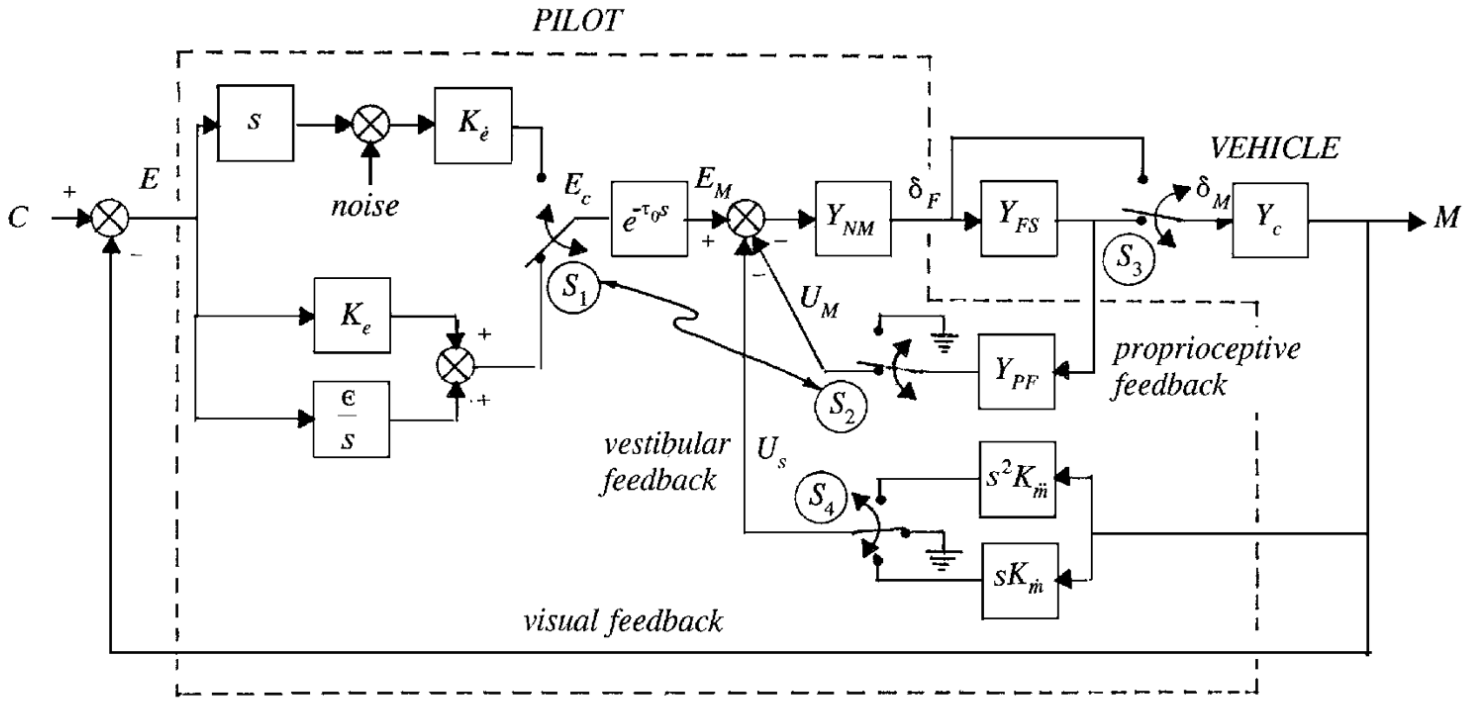
\includegraphics[width=0.8\linewidth]{figures/Introduction/Screen_Shot_2018-07-31_at_11_21_44_AM.png}
        \caption[The Structural Model of the Human Pilot]{The Structural Model of the Human Pilot, from~\citet{hess_unified_1997}.}
        \label{figure:structuralmodel}
    \end{center}
\end{figure}

While the crossover model was very successful in predicting pilot behavior, it did not attempt ``to describe the underlying structure which contributes to human pilot dynamics~\citep{hess_structural_1980}.''
For this reason, the Structural Model is of interest due to the incorporation of multiple sensory channels and models of visual acuity and the time-varying human pilot~\citep{hess_modeling_2009}.
The Structural Model includes the effects of the neuromuscular system, the force-feel characteristics of the input device, and the contributions of proprioceptive, vestibular, and visual feedback, see Figure~\ref{figure:structuralmodel}.
One of the key strengths of the Structural Model is the relatively small number of free parameters that need to be set to predict pilot performance.
The model has been used in predicting and evaluating handling qualities and pilot-induced oscillation rating levels for helicopters, the Boeing 747, the Lockheed C-5A, and twin ducted-fan aircraft~\citep{hess_analytical_2013, andreea-irina_prediction_2014, grant_handling_2015}.
Hess has also used the model to investigate how pilot control characteristics change with time due to flight anomalies, changing flight dynamics, and sudden increases in task demand~\citep{hess_modeling_2009, hess_modeling_2016}.
The results of this model have been compared to the results of a human-in-the-loop simulation for a well-trained subject and showed good comparison~\citep{hess_modeling_2016}.
Recent work from Bachelder et al. has included modifications to the Structural Model to link pilot performance and workload, and to enable the modeling of pulsive pilot behavior~\citep{bachelder_modeling_2017, bachelder_linking_2018}.

\subsection{Summary}
Augmented feedback has been used in a large variety of motor control tasks and has generally been found to improve performance.
Until recently, however, only simple tasks such as physical movements or low-dimensional pursuit tasks have been investigated.
More recent works, including the lane-keeping task by \citeauthor{de_groot_effect_2011} and our previous work with the SAFER task, have indicated that concurrent bandwidth feedback can also be quite effective for complex tasks~\citep{karasinski_real-time_2017}.
Unlike simple tasks, in which the guidance hypothesis dominates when feedback is removed, there is some evidence that concurrent bandwidth feedback can be removed after training complex tasks without a loss of performance.
The decrease in required learning time, improved maximum performance, and decreased workload seen in the SAFER task show that concurrent bandwidth feedback may prove to be most useful very early in training when subjects are first exposed to complex, highly dynamic tasks.
As concurrent bandwidth feedback can improve performance for complex tasks without an increase in workload, it may prove a useful technique for training other complex manual control tasks.

There has been considerable improvement in the field of pilot modeling since McRuer's crossover model, especially with models that incorporate human physiology.
The Structural Model, in particular, has been very effective in predicting pilot performance, handling qualities, pilot-induced oscillation rating levels, and workload for a variety of system dynamics.
None of these pilot models, however, are able to include the effects of concurrent bandwidth feedback.
The performance improving potential of this feedback make this a compelling feature to be incorporated into a pilot model.

% This literature review covered the development of the augmented feedback, focusing on examples of concurrent and bandwidth feedback.
% Extra focus was spent on cases where augmented feedback techniques were applied to aerospace related tasks.
% Additionally, this review covered human performance models applied to piloted aircraft and flight-like tasks.

\section{Research Questions}
\label{sec:intro_questions}
% To this end, this proposed research includes two research aims.
We set out to accomplish two aims with the research included in this dissertation.
These aims build on each other, starting with a compensatory tracking task, extending to surface electromyography and aircraft flight tasks, and finishing with a theoretical model.
This dissertation contains the results of human-in-the-loop subject testing experiments which were designed to understand the effects of concurrent bandwidth feedback.
Using the data from these experiments, the Structural Model was modified to integrate the effects of this feedback into a human performance model.
To investigate the two aims outlined below, we completed four experiments and the development of a model.

\begin{description}[align=left]
    \item [Aim One] Investigate the effects of concurrent bandwidth feedback on human performance and workload in complex manual control tasks.
    \item [Aim Two] Extend the Structural Model of the human pilot to include the effects of concurrent bandwidth feedback.
\end{description}

There are several research questions that we are interested in answering by completing these aims, which include:
\begin{enumerate}
    \item Can concurrent bandwidth feedback (CBF) improve human performance in complex manual control tasks?
          \begin{enumerate}
              \item Can CBF reduce the required training time to peak performance?
              \item Can CBF be removed after reaching peak performance without reducing subject performance (i.e., does the guidance hypothesis not hold)?
                    %   \item Does CBF improve performance in transfer of training tasks?
              \item Can performance be increased without increasing workload?
          \end{enumerate}
    \item Can we develop a model of human performance that includes the effects of concurrent bandwidth feedback?
          \begin{enumerate}
              \item Can we use this model to estimate operational limits?
          \end{enumerate}
\end{enumerate}

\section{Summary}
We have introduced our goals and motivation for the design and use of concurrent bandwidth feedback.
The background for the experimental work has been described and the open research questions that we explore in this work have been summarized.
In the following chapters, we first present a systematic assessment of current and upcoming human automation/robotic integration technologies and research topics (Chapter~\ref{chapter:tradestudy}), then report on four experiments involving augmented feedback (Chapters~\ref{chap:3dtracking}-\ref{chapter:bandwidthstudy}), propose a theoretical model which explains the observed effects of the feedback (Chapter~\ref{chapter:modeling}), and summarize our findings and proposed future work (Chapter~\ref{chap:conclusion}).
